\section{Background}
\label{sec:background}
In this section, we present background information about the maintenance of
Linux kernel stable versions, the potential benefits of introducing
automation into the stable kernel maintenance process, and the challenges
that the maintenance of Linux kernel stable versions poses for automation
via machine learning.

\subsection{Context}
\label{sec:context}
Linux kernel development is carried out according to a hierarchical model,
with Linus Torvalds, who has ultimate authority about which
patches are accepted into the kernel, at the root and patch {\em authors} at the
leaves. A patch author is anyone who wishes to make a contribution to the
kernel, to fix a bug, add a new functionality, or improve the coding
style. Authors submit their patches by email to {\em maintainers}, who
commit the changes to their git trees and submit pull requests up the
hierarchy. In this work, we are mostly concerned with the maintainers, who
have the responsibility of assessing the correctness and usefulness of the
patches that they receive. Part of this responsibility involves determining
whether a patch is stable-relevant, and annotating it accordingly.

The Linux kernel provides a number of guidelines to help maintainers
determine whether a patch should be annotated for propagation to stable
kernels \cite{stabledoc}. These are summarized as follows:
\begin{itemize}[leftmargin=0.4cm]
\item It cannot be bigger than 100 lines.
\item It must fix a problem that causes a build error, an oops, a hang, data corruption,
a real security issue, or some ``oh, that’s not good'' issue.
% \item It must fix a real bug that bothers people.
\end{itemize}
These criteria may be simple, but are open
to interpretation. For example, even the criterion about patch size, which
seems unambiguous, is only satisfied by 93\% of the patches found in the
stable versions based on Linux v3.0 to v4.13, as of September
2017. 

\subsection{Potential}

We consider how to estimate the benefit that automatic identification of
stable-relevant patches can provide. To understand the potential benefit,
we examine the percentage of all mainline commits that are propagated to
stable kernels across different kernel subsystems and the percentage of
these that are annotated with the Cc: stable tag.  We focus on the 12
directories for which more than 500 mainline commits were propagated
to stable kernels between Linux v3.0 (July 2011) and Linux v4.12 (July
2017).  Figure \ref{pctprop} shows the percentage of all mainline commits
that are propagated to stable kernels for these 12 directories.  We observe
that there is a large variation in these values.  Comparing directories
with similar purposes, 4\% of {\tt arch/arm} (ARM hardware support) commits
are propagated, while 10\% of {\tt arch/x86} (x86 hardware support) commits
are propagated, and 6-8\% of the {\tt scsi}, {\tt gpu} and {\tt net} driver
commits are propagated; while 17\% of {\tt usb} driver commits are
propagated.\footnote{The {\tt usb} driver maintainer is also a stable kernel
  maintainer.}  While the need for propagating commits to stable kernels
may depend on the quality and maturity of the given code, the wide
variation in the propagation rates for similar kinds of code suggests that
relevant commits may be missed.

\begin{figure}
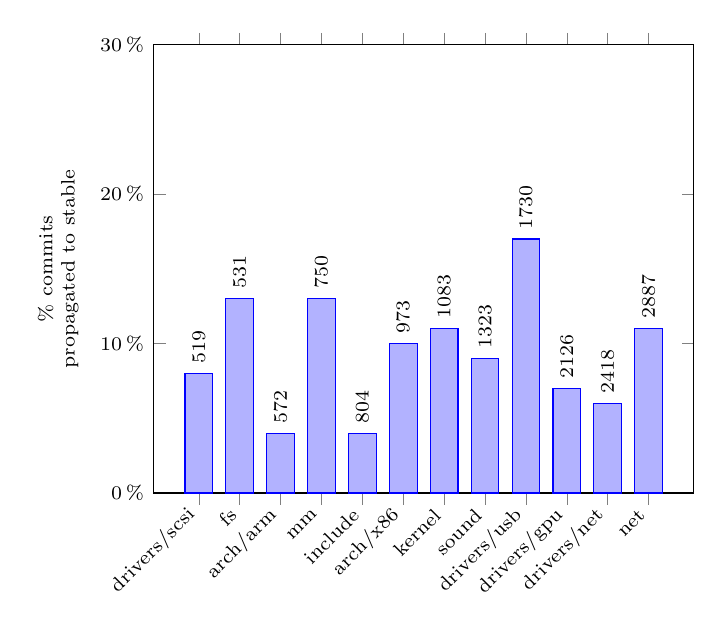
\begin{tikzpicture}
\begin{axis}[ybar,xtick=data,ticklabel style = {font=\scriptsize},
 label style = {font=\scriptsize},
 x tick label style={rotate=45,anchor=east, yshift=-0.01em},
ylabel={\begin{tabular}{c}\% commits\\propagated to stable\end{tabular}},
yticklabel=\pgfmathprintnumber{\tick}\,$\%$,
        ymin=0,
        ymax=30,
symbolic x
    coords={drivers/scsi,fs,arch/arm,mm,include,arch/x86,kernel,sound,drivers/usb,drivers/gpu,drivers/net,net}]
\addplot coordinates
{(drivers/scsi,                   8)
(fs,                             13)
(arch/arm,                       4)
(mm,                             13)
(include,                        4)
(arch/x86,                       10)
(kernel,                         11)
(sound,                          9)
(drivers/usb,                    17)
(drivers/gpu,                    7)
(drivers/net,                    6)
(net,                            11)};

\node[below,rotate=90,anchor=west] at (axis cs:drivers/scsi,8) {\scriptsize 519};
\node[below,rotate=90,anchor=west] at (axis cs:fs,13) {\scriptsize 531};
\node[below,rotate=90,anchor=west] at (axis cs:arch/arm,4) {\scriptsize 572};
\node[below,rotate=90,anchor=west] at (axis cs:mm,13) {\scriptsize 750};
\node[below,rotate=90,anchor=west] at (axis cs:include,4) {\scriptsize 804};
\node[below,rotate=90,anchor=west] at (axis cs:arch/x86,10) {\scriptsize 973};
\node[below,rotate=90,anchor=west] at (axis cs:kernel,11) {\scriptsize 1083};
\node[below,rotate=90,anchor=west] at (axis cs:sound,9) {\scriptsize 1323};
\node[below,rotate=90,anchor=west] at (axis cs:drivers/usb,17) {\scriptsize 1730};
\node[below,rotate=90,anchor=west] at (axis cs:drivers/gpu,7) {\scriptsize 2126};
\node[below,rotate=90,anchor=west] at (axis cs:drivers/net,6) {\scriptsize 2418};
\node[below,rotate=90,anchor=west] at (axis cs:net,11) {\scriptsize 2887};

\end{axis}
\end{tikzpicture}
\caption{Percentage of mainline commits propagated to stable kernels for
  the 12 directories with the most stable commits. The number above each bar
  indicates the number of propagated commits.}
\label{pctprop}
\end{figure}

Figure \ref{pctcom} shows the percentage of mainline commits propagated to
stable kernels that contain the Cc: stable tag, for the same set of kernel
directories.  The rate is very low for {\tt drivers/net} and {\tt net},
which are documented to have their own procedure \cite{stabledoc}.  The
others mostly range from 60\% to 85\%.  Commits in stable kernels that do
not contain the tag are commits that the stable maintainers have identified
on their own or that they have received via other non-standard channels.
This represents further work that can be saved by an automatic labeling
approach.

\begin{figure}
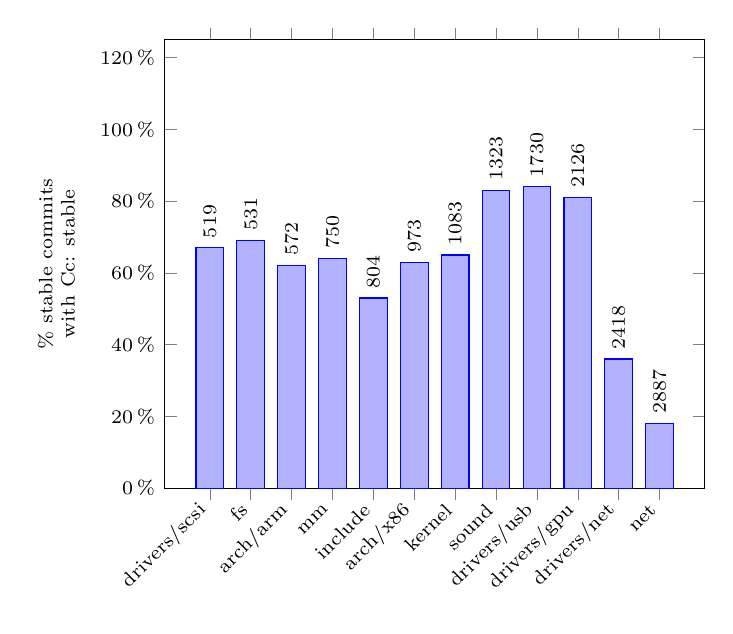
\begin{tikzpicture}
\begin{axis}[ybar,xtick=data,ticklabel style = {font=\scriptsize},
 label style = {font=\scriptsize},
 x tick label style={rotate=45,anchor=east, yshift=-0.01em},
ylabel={\begin{tabular}{c}\% stable commits\\with Cc: stable\end{tabular}},
yticklabel=\pgfmathprintnumber{\tick}\,$\%$,
        ymin=0,
        ymax=125,
symbolic x
    coords={drivers/scsi,fs,arch/arm,mm,include,arch/x86,kernel,sound,drivers/usb,drivers/gpu,drivers/net,net}]
\addplot coordinates
{(drivers/scsi,                   67)
(fs,                             69)
(arch/arm,                       62)
(mm,                             64)
(include,                        53)
(arch/x86,                       63)
(kernel,                         65)
(sound,                          83)
(drivers/usb,                    84)
(drivers/gpu,                    81)
(drivers/net,                    36)
(net,                            18)};

\node[below,rotate=90,anchor=west] at (axis cs:drivers/scsi,67) {\scriptsize 519};
\node[below,rotate=90,anchor=west] at (axis cs:fs,69) {\scriptsize 531};
\node[below,rotate=90,anchor=west] at (axis cs:arch/arm,62) {\scriptsize 572};
\node[below,rotate=90,anchor=west] at (axis cs:mm,64) {\scriptsize 750};
\node[below,rotate=90,anchor=west] at (axis cs:include,53) {\scriptsize 804};
\node[below,rotate=90,anchor=west] at (axis cs:arch/x86,63) {\scriptsize 973};
\node[below,rotate=90,anchor=west] at (axis cs:kernel,65) {\scriptsize 1083};
\node[below,rotate=90,anchor=west] at (axis cs:sound,83) {\scriptsize 1323};
\node[below,rotate=90,anchor=west] at (axis cs:drivers/usb,84) {\scriptsize 1730};
\node[below,rotate=90,anchor=west] at (axis cs:drivers/gpu,81) {\scriptsize 2126};
\node[below,rotate=90,anchor=west] at (axis cs:drivers/net,36) {\scriptsize 2418};
\node[below,rotate=90,anchor=west] at (axis cs:net,18) {\scriptsize 2887};

\end{axis}
\end{tikzpicture}
\caption{Percentage of mainline commits propagated to stable kernels that
  contain a Cc: stable tag for the 12 directories with the most mainline
  commits propagated to stable kernels. The number above each bar indicates
the number of propagated commits.}
\label{pctcom}
\end{figure}

\subsection{Challenges for Machine Learning}
\label{sec:challenges}

Stable patch identification poses some unique challenges for machine learning.
These include the kind of information available in a Linux kernel patch and the
diversity in the reasons why patches are or are not selected for application to stable
kernels.

First, Linux kernel commit logs are written free-form. While maintainers
are asked to add a ``Cc: stable@vger.kernel.org'' tag to commits that
should be propagated to stable versions, they may neglect to do this.  
% Our
% goal is to identify stable-relevant commits for which adding this tag has
% been overlooked, and thus we ignore this information \jl{Maybe this
%   sentence is not needed here; it is more about our dataset. which comes
%   later.}. 
  Patches also contain a combination of text, represented by the
commit log, and code, represented by the enumeration of the changed
lines. Code is structured differently than text, and thus we need to
construct a representation that enables machine learning algorithms to
detect relevant properties.

Second, some patches applied to stable kernels are not bug fixing
patches. The stable documentation itself stipulates that patches adding new
device identifiers are also acceptable. Such patches represent a very simple form
of new functionality, implemented as an array element initialization, but they are
allowed in stable kernels because they are unlikely to cause problems for users of
stable kernels and may enable the use of the stable kernel with new device variants.
% These patches have a common structure and are easily recognized, and thus should
% not pose a significant challenge for machine learning. 
Another reason that a non bug
fixing patch may be introduced into a stable kernel is that a subsequent bug
fixing patch depends on it. 
These non bug fixing patches, which typically perform
refactorings, should satisfy the criteria of being small and obviously correct, but
may have other properties that differ from those of bug-fixing patches. They may
thus introduce apparent inconsistencies into the machine learning process.

Finally, some patches may perform bug fixes, but may be correctly not propagated to
stable. One reason is that some parts of the code change so rapidly that the patch
does not apply cleanly to any stable version. Another reason is that the bug was
introduced since the most recent mainline release, and thus does not appear in any
stable version.

As the decision of whether to apply a patch to a stable kernel depends in part
on factors external to the patch itself, we cannot hope to achieve a perfect solution
based on applying machine learning to patches alone. 
% Still, stable-kernel maintainers
% have reported to us that they are able to check likely stable-relevant patches
% quickly (e.g., 32 in around 20 minutes).\footnote{Greg Kroah Hartman, private communication, April 28, 2017}. 
Still, we believe that we can effectively
complement existing practice by orienting stable-kernel maintainers towards
likely stable-relevant commits that they may have overlooked, even though
the above issues introduce the risk of some false negatives and false positives.

